\section{Grundlagen der Datenanalyse}

Mathematisch ausgedrückt besteht eine Zeitreihe (im englischen auch \enquote{time series} genannt) aus einer endlichen Menge an zeitlich aufsteigend sortierten Messwerten $x_{t_1},x_{t_2},...,x_{t_T};  x_{t_k} \in \mathbb{R}^n, k=1,2,...,T$, wofür $t_1 < t_2 < t_T $ gilt.\footcite[Vgl.][1]{Deistler.2018b} Zeitreihendaten sind in verschiedenen Feldern zu finden, beispielsweise im Bereich der Aktienmärkte, wo die Preise der einzelnen Kurse abgebildet werden, im Bereich der Gesundheitsforschung, wo die Ansteckungsrate ansteckender Krankheiten wie Covid-19 verfolgt wird oder im Bereich der Sozialwissenschaften, in welchen der Verlauf von Geburtsraten über die Zeit analysiert werden soll.\footcite[Vgl.][1]{Shumway.2017b} In \autoref{abb:BeispielZeitreihe} findet sich beispielhaft die Zeitreihe der verimpften Dosen des COVID-19 Impfstoffes im Januar 2021.

\begin{figure}[H]
\centering
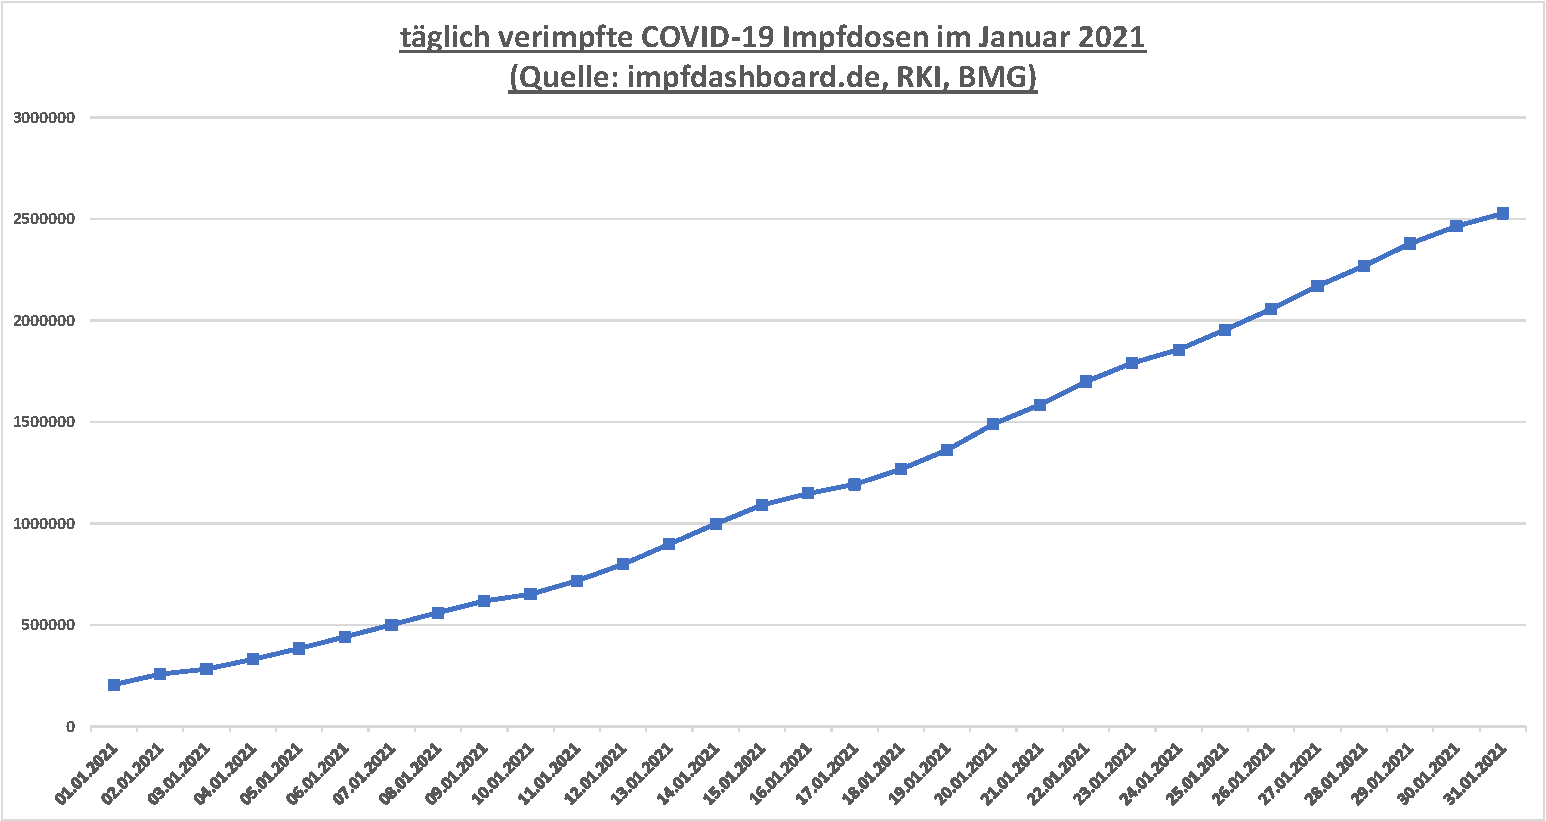
\includegraphics[width=\textwidth]{graphics/Beispiel-Zeitreihe.pdf}
\caption{Beispielhafte Zeitreihe aus dem Januar 2021}
\label{abb:BeispielZeitreihe}
\end{figure}

Die möglichen Anwendungen in der Informatik sind ebenfalls vielzählig. So können über virtuelle oder physikalische Sensoren Messwerte, wie beispielsweise die CPU Auslastung eines gegebenen Servers über die Zeit oder Temperaturmessungen eines \ac{IoT} Gerätes über die Zeit gemacht und gespeichert werden.

Ein wichtiges Merkmal von Zeitreihen ist die Distanz zwischen den Messwerten, im Sinne der Messfrequenz, in welcher Daten betrachtet werden. \Todo{belegen} Ist eine Zeitreihe äquidistant, wurde mit gleichbleibender Frequenz gemessen und die zeitliche Distanz zwischen einzelnen Messwerten ist gleich. Für die in dieser Arbeit diskutierten Auswertungsarten wird eine Äquidistanz der gemessenen Daten angenommen, da andernfalls ein Bias bei der Analyse nicht ausgeschlossen werden kann. Gleichfalls ist es technisch möglich einzelne, nicht äquidistante Messwerte auszusortieren. Die in \autoref{abb:BeispielZeitreihe} abgebildete Zeitreihe ist äquidistant, da die Werte einmal am Tag gesammelt erhoben wurden.


\Todo{Definition Zeitreihendaten}
\Todo{Definition Datenanalyse}

\Todo{Grafik Data Analytics Pipeline}



\subsection{Arten der Auswertung}
\subsubsection{Median}
\subsubsection{Anomaliedetektion}
\subsubsection{Schwellwertüberschreitung}
\subsubsection{Trenderkennung/gleitender Durchschnitt}

\subsection{Vorbestehende Referenzarchitekturen}
Zur Verarbeitung von Streamingdaten gibt es bereits zwei bestehende, im Umfeld der von der Apache Foundation betreuten Streamingprodukten entstandenen Referenzarchitekturen. 



\subsection{Echtzeitverarbeitung}
https://blogs.oracle.com/analytics/the-half-life-of-data-and-the-role-of-analytics
\subsubsection{Streamanalyse}
\begin{itemize}
\item AWS Kinesis Data Analytics/Stream
\item AWS Lambda
\end{itemize}

\subsection{Datenbankseitige Verarbeitung}
\subsubsection{Datenbankabfragen}
\begin{itemize}
\item Timestream
\item Redshift
\item Athena
\item Elasticsearch
\end{itemize}

\subsubsection{Externe Analyse}
\begin{itemize}
\item Amazon EMR
\item Amazon Glue
\item AWS Lake Formation
\end{itemize}




Source -> Stream ingestion -> Stream storage -> Stream processing -> Destination

Talkingpoints gegen Streaming onprem:
Difficult to set up, Difficult to achieve high availability,
Error prone and complex to manage,
Tricky to scale, Integration requires development,Expensive to maintain

Amazon Kinesis Data Streams - Daten verfügbar in 70 Milisekunden



Amazon Kinesis Data Analytics


\subsubsection{Brokeranalyse}

\begin{itemize}
\item AWS IoT Analytics
\end{itemize}